% !TEX root = ../main.tex

% 报告主体

%%%
%---------------------------------------------------------------------
% 实验
\clearpage
\JMSection{实验过程}
\subsection{系统预热和仪器调节}
\begin{itemize}
    \item[1.] 检查主体单元光路的机械安装和调整。
    
    \item[2.] 借助磁针,调节导轨,使主体装置的光轴与地磁场水平方向平行。
    
    \begin{ubox}
        {如何调节?判断方向平行的依据是什么?}
        将磁针放置在主体装置附近,确保磁针的指向与光轴方向一致。磁针的N极指向地磁场的北极方向,S极指向地磁场的南极方向。光轴与磁针的指向平行时,即可认为光轴与地磁场水平方向平行。
    \end{ubox}
   
    
    \item[3.] 检查各联线是否正确。将电源前面板上的“垂直”、“水平”和辅助源前面板“扫场幅度”旋钮调到最小。
    \item[4.] 接通电源,加热铷光谱灯和吸收池,约30分钟后,灯温、池温指示灯点亮,实验装置进入工作状态。从铷灯后面小圆窗口观察,灯泡应发出玫瑰紫色的光。
    \begin{ubox}
        {温度控制在多少时,信号最大?对于$^{87}$Rb和$^{85}$Rb,情况是否一样?}
        铷光谱灯的温度通常控制在90℃左右,吸收池的温度控制在55℃左右。对于$^{87}$Rb和$^{85}$Rb,实验室通常使用相同温度设置。
    \end{ubox}

\end{itemize}

\subsection{观察光抽运信号,并分析讨论}

\begin{enumerate}
    \item 调出光抽运信号,细调扫场幅度、偏振片与玻片夹角、垂直磁场电流及光路上各元件位置等,使信号达到最大;
    
    \item 利用磁针,预先判断并记录辅助源前面板水平磁场、垂直磁场、扫场方向控制开关代表的方向状态,与地磁场方向是否同向或反向。
    
    \item 观察和记录不同磁场情况:

        (a)水平、垂直磁场为零时,扫场与地磁场同向或反向,并改变扫场大小;
        
       (b)扫场与地磁场同向时,分别改变水平和垂直磁场的大小和方向;
        
        (c)扫场与地磁场反向时,重复(b);
        
        (d)改用三角波扫场方式,重复(b)(c)实验步骤;
        
       (e)改用外接扫场方式(将辅助源后面板扫场开关置"外"),信号发生器选择方波或三角波,分别改变信号输出的幅度和扫描速度等以上所有的光抽运信号,并分析形成原因。
    \end{enumerate}

\subsubsection{(a)部分结果}

 \begin{figure}[H]
    \centering
    \begin{minipage}[b]{0.45\linewidth}
        \centering
        \includegraphics[width=\linewidth]{振幅小-扫场与地磁场同向.png}
        \caption{振幅小-扫场与地磁场同向}
        \label{fig:same_small}
    \end{minipage}
    \hfill
    \begin{minipage}[b]{0.45\linewidth}
        \centering
        \includegraphics[width=\linewidth]{振幅最大-扫场与地磁场同向.png}
        \caption{振幅最大-扫场与地磁场同向}
        \label{fig:same_large}
    \end{minipage}

    \label{fig:same_direction}
\end{figure}

\begin{figure}[H]
    \centering
    \begin{minipage}[b]{0.45\linewidth}
        \centering
        \includegraphics[width=\linewidth]{振幅小-扫场与地磁场反向.png}
        \caption{振幅小-扫场与地磁场反向}
        \label{fig:opposite_small}
    \end{minipage}
    \hfill
    \begin{minipage}[b]{0.45\linewidth}
        \centering
        \includegraphics[width=\linewidth]{振幅最大-扫场与地磁场反向.png}
        \caption{振幅最大-扫场与地磁场反向}
        \label{fig:opposite_large}
    \end{minipage}

    \label{fig:opposite_direction}
\end{figure}


当外加扫场与地磁场方向相同时,总磁场方向与地磁场一致。此时,铷原子能级的塞曼分裂随扫场强度增加而加剧,光抽运效应增强,原子对光的吸收效率提高,检测信号强度增大。

相反,当扫场方向与地磁场相反时,总磁场方向反转。尽管铷原子能级仍随扫场增强而分裂,但原子对探测光的吸收能力降低,导致信号强度减弱。



\subsubsection{(b)部分结果}

\begin{figure}[H]
    \centering
    \begin{minipage}[b]{0.45\linewidth}
        \centering
        \includegraphics[width=\linewidth]{水平磁场off,电流0.020A;垂直磁场off,电流0.057A.png}
        \caption{水平磁场关闭(0.020A),垂直磁场关闭(0.057A)}
        \label{fig:both_off}
    \end{minipage}
    \hfill
    \begin{minipage}[b]{0.45\linewidth}
        \centering
        \includegraphics[width=\linewidth]{水平磁场off,电流0.206A;垂直磁场on,电流0.136A.png}
        \caption{水平磁场关闭(0.206A),垂直磁场开启(0.136A)}
        \label{fig:h_off_v_on}
    \end{minipage}

    \label{fig:horizontal_off}
\end{figure}

\begin{figure}[H]
    \centering
    \begin{minipage}[b]{0.45\linewidth}
        \centering
        \includegraphics[width=\linewidth]{水平磁场on,电流0.067A;垂直磁场off,电流0.025A.png}
        \caption{水平磁场开启(0.067A),垂直磁场关闭(0.025A)}
        \label{fig:h_on_v_off}
    \end{minipage}
    \hfill
    \begin{minipage}[b]{0.45\linewidth}
        \centering
        \includegraphics[width=\linewidth]{水平磁场on,电流0.084A;垂直磁场on,电流0.212A.png}
        \caption{水平磁场开启(0.084A),垂直磁场开启(0.212A)}
        \label{fig:both_on}
    \end{minipage}

    \label{fig:horizontal_on}
\end{figure}
实验数据显示,调节水平方向电流大小时,随着水平电流的改变,信号波形会发生偏移,且强度分布不再均匀。
在调节垂直磁场时,会影响到地磁场垂直分量对于信号的影响,具体体现为,在测量时会逐步找到一个信号最大的峰值。



\subsubsection{(c)部分结果}

\begin{figure}[H]
    \centering
    \begin{minipage}[b]{0.45\linewidth}
        \centering
        \includegraphics[width=\linewidth]{水平磁场off,电流0.099A;垂直磁场off,电流0.070A.png}
        \caption{水平磁场关闭(0.099A),垂直磁场关闭(0.070A)}
        \label{fig:h_off_v_off}
    \end{minipage}
    \hfill
    \begin{minipage}[b]{0.45\linewidth}
        \centering
        \includegraphics[width=\linewidth]{水平磁场off,电流0.105A;垂直磁场on,电流0.067A.png}
        \caption{水平磁场关闭(0.105A),垂直磁场开启(0.067A)}
        \label{fig:h_off_v_on}
    \end{minipage}

    \label{fig:horizontal_off}
\end{figure}

% 第二组:水平磁场开启的情况
\begin{figure}[H]
    \centering
    \begin{minipage}[b]{0.48\linewidth}
        \centering
        \includegraphics[width=\linewidth]{水平磁场on,电流0.066A;垂直磁场on,电流0.082A.png}
        \caption{水平磁场开启(0.066A),垂直磁场开启(0.082A)}
        \label{fig:h_on_v_on}
    \end{minipage}
    \hfill
    \begin{minipage}[b]{0.48\linewidth}
        \centering
        \includegraphics[width=\linewidth]{水平磁场on,电流0.134A;垂直磁场off,电流0.051A.png}
        \caption{水平磁场开启(0.134A),垂直磁场关闭(0.051A)}
        \label{fig:h_on_v_off}
    \end{minipage}

    \label{fig:horizontal_on}
\end{figure}










\subsubsection{(d)部分结果}
扫场与地磁场反向

\begin{figure}[H]
    \centering
    \begin{minipage}{0.45\textwidth}
        \includegraphics[width=\linewidth]{扫场与地磁场反向;水平磁场off,电流0.165A;垂直磁场off,电流0.226A.png}
        \caption{水平磁场off, 电流0.165A; 垂直磁场off, 电流0.226A}
        \label{fig:img1}
    \end{minipage}
       \hfill
    \begin{minipage}{0.45\textwidth}
        \includegraphics[width=\linewidth]{扫场与地磁场反向;水平磁场off,电流0.203A;垂直磁场on,电流0.171A.png}
        \caption{水平磁场off, 电流0.203A; 垂直磁场on, 电流0.171A}
        \label{fig:img2}
    \end{minipage}
\end{figure}

\begin{figure}[H]
    \centering
    \begin{minipage}{0.45\textwidth}
        \includegraphics[width=\linewidth]{扫场与地磁场反向;水平磁场on,电流0.132A;垂直磁场on,电流0.107A.png}
        \caption{水平磁场on, 电流0.132A; 垂直磁场on, 电流0.107A}
        \label{fig:img3}
    \end{minipage}%
       \hfill
    \begin{minipage}{0.45\textwidth}
        \includegraphics[width=\linewidth]{扫场与地磁场反向;水平磁场on,电流0.243A;垂直磁场off,电流0.146A.png}
        \caption{水平磁场on, 电流0.243A; 垂直磁场off, 电流0.146A}
        \label{fig:img4}
    \end{minipage}
\end{figure}

扫场与地磁场同向

\begin{figure}[H]
    \centering
    \begin{minipage}{0.45\textwidth}
        \includegraphics[width=\linewidth]{扫场与地磁场同向;水平磁场off,电流0.030A;垂直磁场on,电流0.122A.png}
        \caption{水平磁场off, 电流0.030A; 垂直磁场on, 电流0.122A}
        \label{fig:img5}
    \end{minipage}%
       \hfill
    \begin{minipage}{0.45\textwidth}
        \includegraphics[width=\linewidth]{扫场与地磁场同向;水平磁场off,电流0.090A;垂直磁场off,电流0.114A.png}
        \caption{水平磁场off, 电流0.090A; 垂直磁场off, 电流0.114A}
        \label{fig:img6}
    \end{minipage}
\end{figure}

\begin{figure}[H]
    \centering
    \begin{minipage}{0.45\textwidth}
        \includegraphics[width=\linewidth]{扫场与地磁场同向;水平磁场on,电流0.017A;垂直磁场on,电流0.144A.png}
        \caption{水平磁场on, 电流0.017A; 垂直磁场on, 电流0.144A}
        \label{fig:img7}
    \end{minipage}%
       \hfill
    \begin{minipage}{0.45\textwidth}
        \includegraphics[width=\linewidth]{扫场与地磁场同向;水平磁场on,电流0.052A;垂直磁场off,电流0.108A.png}
        \caption{水平磁场on, 电流0.052A; 垂直磁场off, 电流0.108A}
        \label{fig:img8}
    \end{minipage}
\end{figure}

幅值偏大和偏小

\begin{figure}[H]
    \centering
    \begin{minipage}{0.45\textwidth}
        \includegraphics[width=\linewidth]{水平磁场0.106A,垂直磁场0.041A,扫场与地磁场反向,幅值偏大.png}
        \caption{水平磁场0.106A, 垂直磁场0.041A, 反向, 幅值偏大}
        \label{fig:img9}
    \end{minipage}%
       \hfill
    \begin{minipage}{0.45\textwidth}
        \includegraphics[width=\linewidth]{水平磁场0.106A,垂直磁场0.041A,扫场与地磁场反向,幅值偏小.png}
        \caption{水平电流0.106A, 垂直磁场0.041A, 反向, 幅值偏小}
        \label{fig:img10}
    \end{minipage}
\end{figure}

\begin{figure}[H]
    \centering
    \begin{minipage}{0.45\textwidth}
        \includegraphics[width=\linewidth]{水平磁场0.106A,垂直磁场0.041A,扫场与地磁场同向,幅值偏大.png}
        \caption{水平磁场0.106A, 垂直磁场0.041A, 同向, 幅值偏大}
        \label{fig:img11}
    \end{minipage}%
       \hfill
    \begin{minipage}{0.45\textwidth}
        \includegraphics[width=\linewidth]{水平磁场0.106A,垂直磁场0.041A,扫场与地磁场同向,幅值偏小.png}
        \caption{水平磁场0.106A, 垂直磁场0.041A, 同向, 幅值偏小}
        \label{fig:img12}
    \end{minipage}
\end{figure}



\subsubsection{(e)部分结果}



扫场与地磁场反向

\begin{figure}[H]
    \centering
    \begin{minipage}{0.45\textwidth}
        \includegraphics[width=\linewidth]{扫场与地磁场反向;水平磁场off,电流0.110A;垂直磁场off,电流0.165A.png}
        \caption{水平磁场off,电流0.110A;垂直磁场off,电流0.165A}
        \label{fig:img1}
    \end{minipage}%
         \hfill
    \begin{minipage}{0.45\textwidth}
        \includegraphics[width=\linewidth]{扫场与地磁场反向;水平磁场off,电流0.119A;垂直磁场on,电流0.149A.png}
        \caption{水平磁场off,电流0.119A;垂直磁场on,电流0.149A}
        \label{fig:img2}
    \end{minipage}
\end{figure}

\begin{figure}[H]
    \centering
    \begin{minipage}{0.45\textwidth}
        \includegraphics[width=\linewidth]{扫场与地磁场反向;水平磁场on,电流0.018A;垂直磁场on,电流0.183A.png}
        \caption{水平磁场on,电流0.018A;垂直磁场on,电流0.183A}
        \label{fig:img3}
    \end{minipage}%
         \hfill
    \begin{minipage}{0.45\textwidth}
        \includegraphics[width=\linewidth]{扫场与地磁场反向;水平磁场on,电流0.084A;垂直磁场off,电流0.169A.png}
        \caption{水平磁场on,电流0.084A;垂直磁场off,电流0.169A}
        \label{fig:img4}
    \end{minipage}
\end{figure}

扫场与地磁场同向

\begin{figure}[H]
    \centering
    \begin{minipage}{0.45\textwidth}
        \includegraphics[width=\linewidth]{扫场与地磁场同向;水平磁场off,电流0.049A;垂直磁场off,电流0.178A.png}
        \caption{水平磁场off,电流0.049A;垂直磁场off,电流0.178A}
        \label{fig:img5}
    \end{minipage}%
         \hfill
    \begin{minipage}{0.45\textwidth}
        \includegraphics[width=\linewidth]{扫场与地磁场同向;水平磁场off,电流0.074A;垂直磁场on,电流0.161A.png}
        \caption{水平磁场off,电流0.074A;垂直磁场on,电流0.161A}
        \label{fig:img6}
    \end{minipage}
\end{figure}
\begin{figure}[H]
    \centering
    \begin{minipage}{0.45\textwidth}
        \includegraphics[width=\linewidth]{扫场与地磁场同向;水平磁场on,电流0.056A;垂直磁场off,电流0.144A.png}
        \caption{水平磁场on,电流0.056A;垂直磁场off,电流0.144A}
        \label{fig:img7}
    \end{minipage}%
         \hfill
    \begin{minipage}{0.45\textwidth}
        \includegraphics[width=\linewidth]{扫场与地磁场同向;水平磁场on,电流0.165A;垂直磁场on,电流0.088A.png}
        \caption{水平磁场on,电流0.165A;垂直磁场on,电流0.088A}
        \label{fig:img8}
    \end{minipage}
\end{figure}


幅值偏大和偏小



\begin{figure}[H]
    \centering
    \begin{minipage}{0.45\textwidth}
        \includegraphics[width=\linewidth]{水平磁场off,电流0.063;垂直磁场on,电流0.044A;扫场与地磁场反向,幅值偏大.png}
        \caption{水平磁场off,电流0.063;垂直磁场on,电流0.044A;扫场与地磁场反向,幅值偏大}
        \label{fig:img9}
    \end{minipage}%
         \hfill
    \begin{minipage}{0.45\textwidth}
        \includegraphics[width=\linewidth]{水平磁场off,电流0.063;垂直磁场on,电流0.044A;扫场与地磁场反向,幅值偏小.png}
        \caption{水平磁场off,电流0.063;垂直磁场on,电流0.044A;扫场与地磁场反向,幅值偏小}
        \label{fig:img10}
    \end{minipage}
\end{figure}

\begin{figure}[H]
    \centering
    \begin{minipage}{0.45\textwidth}
        \includegraphics[width=\linewidth]{水平磁场off,电流0.063;垂直磁场on,电流0.044A;扫场与地磁场同向,幅值偏大.png}
        \caption{水平磁场off,电流0.063;垂直磁场on,电流0.044A;扫场与地磁场同向,幅值偏大}
        \label{fig:img11}
    \end{minipage}%
         \hfill
    \begin{minipage}{0.45\textwidth}
        \includegraphics[width=\linewidth]{水平磁场off,电流0.063;垂直磁场on,电流0.044A;扫场与地磁场同向,幅值偏小.png}
        \caption{水平磁场off,电流0.063;垂直磁场on,电流0.044A;扫场与地磁场同向,幅值偏小}
        \label{fig:img12}
    \end{minipage}
\end{figure}



\subsubsection{相关分析讨论}

    在本实验中,通过调节各类磁场及实验参数,发现不同条件对光抽运信号的影响如下:
    \begin{itemize}
        \item 扫场与地磁场同向时,能级分裂在原扫场上叠加地磁场后进一步加大,扫场调节过程中零磁场点偏移;光抽运信号仍能观察到,但中心偏离零点;如果未进行磁补偿,可能导致信号不对称或展宽。扫场与地磁场反向时,扫场与地磁场相互抵消,在某一时刻可能恰好出现零磁场点;如果设置合理,此时可观察到对称、明显的双峰结构信号;光抽运效果更显著,有利于研究磁场对抽运过程的影响。

        \item 水平方向磁场的变化对光抽运信号的影响主要体现在是否有信号以及信号是否对称。当水平磁场刚好抵消地磁场的水平分量时,光抽运信号应当在一个扫场周期内出现两次,且是等间隔的;若没有抵消,则两次信号将不会等间隔出现。

        \item 垂直方向的磁场对光抽运影响极大,当垂直磁场为零时(完全抵消地磁场垂直分量),光抽运信号最强、最清晰,且圆偏振光传播方向与量子化轴一致,抽运效率高。当垂直磁场不为零时,会导致量子化轴偏斜,原子“看到”的偏振变成非纯净圆偏振;会造成抽运方向混乱、跃迁通道混合,信号减弱甚至消失。

    \end{itemize}
    
    
    
    于是,我们发现要获得最佳光抽运信号的条件包括以下几点:

    \begin{itemize}
        \item 地磁场的垂直分量会偏转原子的量子化轴,使得激光偏振不再是纯粹的 $\sigma^+$,从而破坏了光抽运的选择性激发过程,降低抽运效率和光抽运信号强度。使用垂直方向的亥姆霍兹线圈精确抵消地磁垂直分量后,系统的偏振条件最优化,抽运效率最高,信号最强。

        \item 当扫场磁场方向与地磁场一致,且扫场幅度控制在合适范围内(能够使能级从简并到分裂并再次简并),可以形成稳定的抽运与去极化过程,信号清晰对称、幅值最大。

        \item 方波扫场有利于观察明显的抽运变化,而三角波扫场则提供更平滑的信号曲线。
        
        \item 外接扫场方式可精确控制扫场波形,有利于高质量信号的提取;扫描速度较慢时,可观察到更清晰的信号结构,有助于定量分析;扫描速度过快时,因铷原子抽运过程存在响应时间,信号展宽或减弱;幅度过小时磁场变化不足,无法形成完整的塞曼结构,信号不明显;

    \end{itemize}









\subsection{测量光抽运时间和弛豫时间}


\subsubsection{实验过程}
   采用外接方波扫场方式,当光抽运信号达到最大时,改变信号发生器信号输出扫描速度,通过直接或拟合方式测出$\tau_1$和$\tau_2$。
\begin{ubox}
 {扫描速度过快能否准确测出弛豫时间?}

在光泵磁共振实验中,扫描速度过快会导致无法准确测量弛豫时间,主要原因在于磁场变化的时间尺度与原子系统的响应时间不匹配。弛豫时间包括描述纵向恢复过程的$\tau_1$和横向退相干过程的$\tau_2$:对于$\tau_2$而言,过快的扫描会使系统未完成弛豫即受干扰,导致共振峰出现展宽、功率加宽或峰值偏移等失真现象;对于$\tau_1$的测量,快速扫描会使透射光信号无法完整反映光抽运的建立/恢复过程,造成测量值$\tau_1^{\mathrm{meas}}$显著小于真实值$\tau_1^{\mathrm{true}}$。为确保测量精度,建议将扫描周期$T$设置为至少5倍$\tau_1$,使系统有充分时间完成弛豫过程。
\end{ubox}

\subsubsection{数据处理}
测量两种弛豫时间 $\tau_1$ 和 $\tau_2$ 的方法如下:

\begin{enumerate}
    \item \textbf{$\tau_1$}:
    通过分析信号的时域衰减曲线,定位相邻的峰值(peak)和谷值(valley),计算两者之间的时间间隔。
    \item \textbf{$\tau_2$}:
    对信号衰减段进行指数函数拟合,模型为 $A(t) = A_0 \mathrm{e}^{-B t} + C$。通过最小二乘法优化拟合参数,取 $\tau_2 = 1 / B$ 。
    \item 直接从示波器导出的数据是使用单位时间(unit time)做单位的,需要用采样率(1000Sa/s)进行修正。
\end{enumerate}


% \begin{figure}[{H}]
%     \centering
%     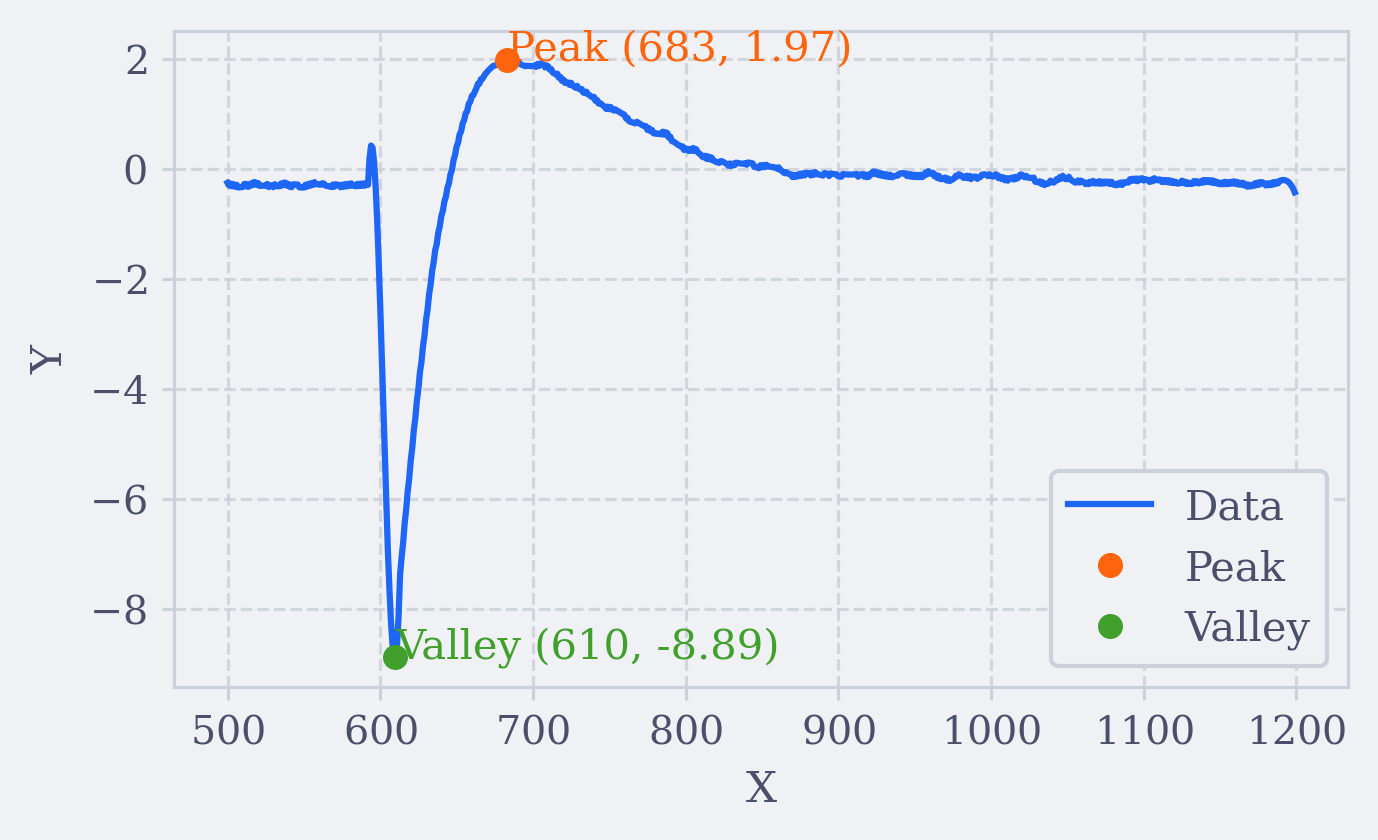
\includegraphics[width=0.6\linewidth]{ex3.png}
%     \caption{弛豫时间峰谷}
%     \label{}
% \end{figure}
% \begin{figure}[{H}]
%     \centering
%     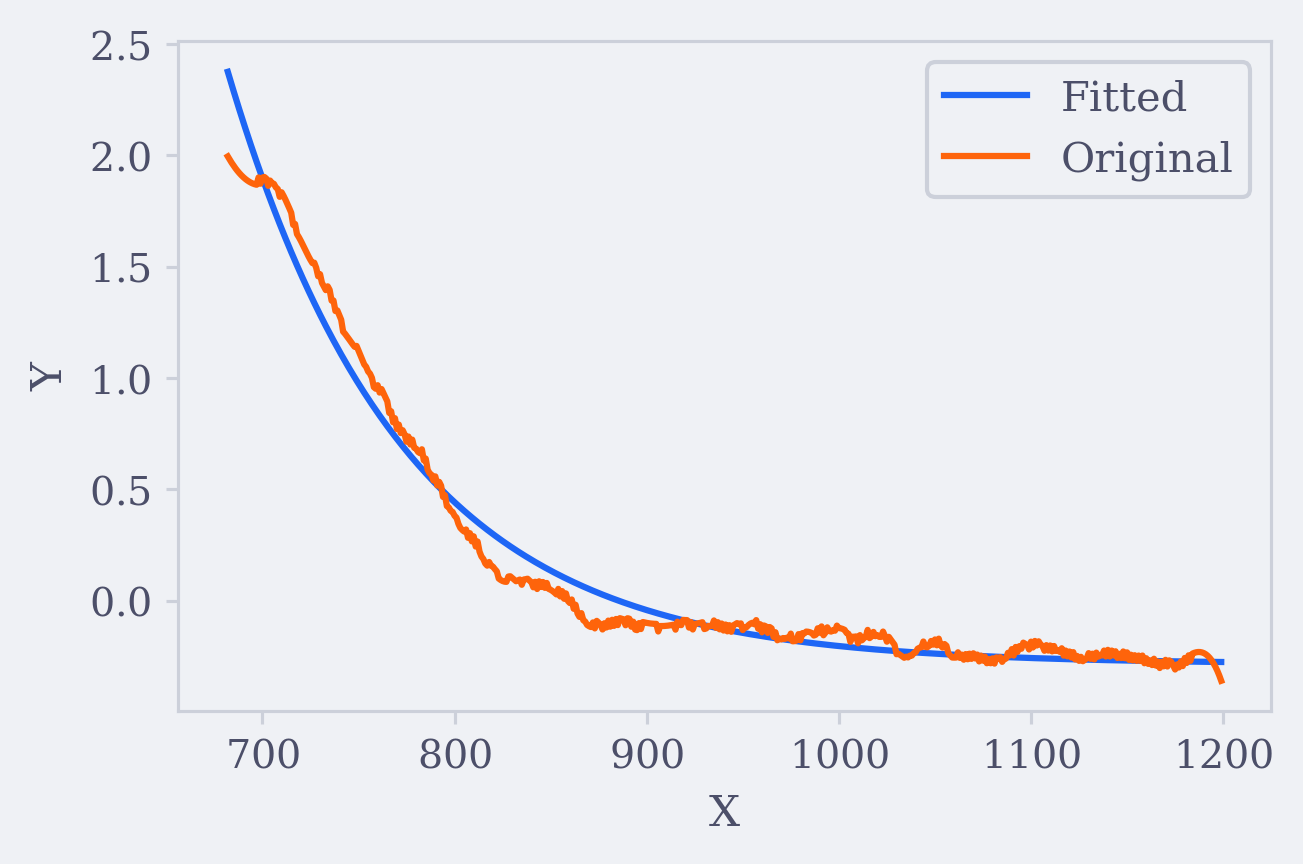
\includegraphics[width=0.6\linewidth]{ex3_1.png}
%     \caption{指数函数拟合}
%     \label{}
% \end{figure}

\begin{figure}[H]
    \centering
    \begin{minipage}[t]{0.48\linewidth}
        \centering
        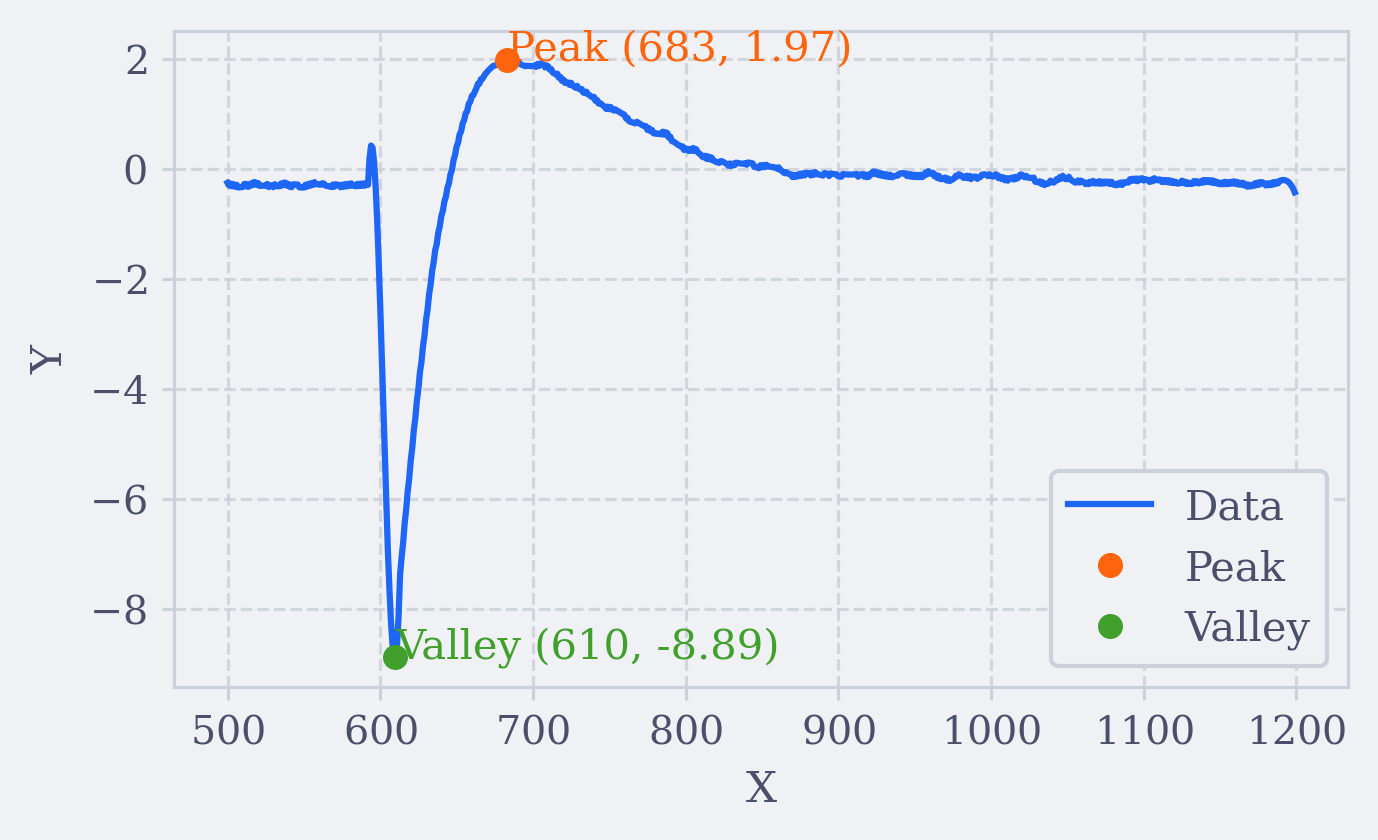
\includegraphics[width=\linewidth]{ex3.png}
        \caption{弛豫时间峰谷}
        \label{fig:relaxation_peaks}
    \end{minipage}
    \hfill
    \begin{minipage}[t]{0.48\linewidth}
        \centering
        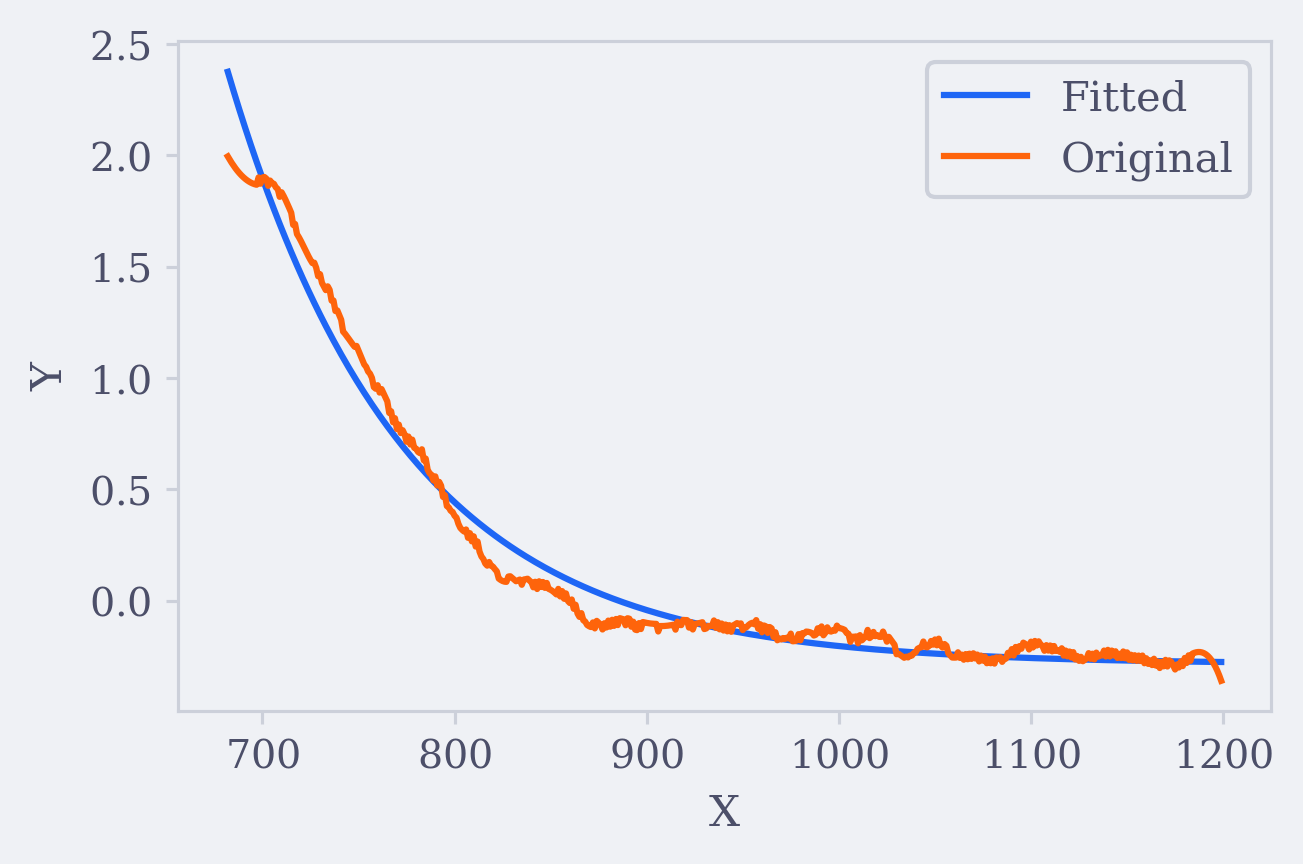
\includegraphics[width=\linewidth]{ex3_1.png}
        \caption{指数函数拟合}
        \label{fig:exponential_fit}
    \end{minipage}
\end{figure}


\begin{table}[htbp]
  \centering
  \caption{指数拟合系数与时间常数测量结果}
  \label{tab:results}
  \begin{tabular}{S[table-format=1.5] 
                  S[table-format=1.2E2] 
                  S[table-format=1.2E2] 
                  S[table-format=4.0]}
    \toprule
    {指数系数 $B$ (unit time)$^{-1}$} & {$\tau_1$ (\si{\second})} & {$\tau_2$ (\si{\second})} & {频率 (\si{\milli\hertz})} \\
    \midrule
    0.01575 & 7.90E-02 & 6.35E-02 & 500  \\
    0.01387 & 6.90E-02 & 7.21E-02 & 600  \\
    0.01472 & 7.50E-02 & 6.79E-02 & 700  \\
    0.01099 & 7.30E-02 & 9.10E-02 & 800  \\
    0.01394 & 7.00E-02 & 7.17E-02 & 900  \\
    0.01477 & 8.00E-02 & 6.77E-02 & 1000 \\
    \midrule
    {均值}  & 7.43E-02 & 7.23E-02 & {--} \\
    {标准差} & 4.55E-03 & 9.67E-03 & {--} \\
    \bottomrule
  \end{tabular}
\end{table}

最终结果如下:
$$\tau_1=7.43 \times 10^{-2} \pm 4.55 \times 10^{-3} \mathrm{s}$$

$$\tau_2=7.23 \times 10^{-2} \pm 9.67 \times 10^{-3} \mathrm{s}$$
\subsubsection{误差分析}
\begin{enumerate}
    \item  采样误差:实验数据是离散采样的,测量出的值可能与真实值有一定偏差,并且对于仪器本身给出的采样率,需要进行修正。
    \item 信号噪声:噪声对于实验结果的影响直接体现在无法确定一个渐近线的值,在使用指数拟合之前,我们尝试了其他寻找$\tau_2$的方法,但是由于信号存在波动,无法找到一个准确的值,最终选择了指数函数拟合。
\end{enumerate}






\subsection{测量 $^{87}\text{Rb}$ 与 $^{85}\text{Rb}$ 的$g_F$ 因子}
\subsubsection{实验过程}
观察磁共振信号,并测量 $^{87}\text{Rb}$ 与 $^{85}\text{Rb}$ 基态超精细结构 $g_F$ 因子。

实验采用三角波信号作为水平扫场信号。在水平磁场线圈中通入特定强度的电流$I$,同时在垂直方向施加射频磁场。首先调整水平线圈产生的磁场方向,使其与扫场信号及地磁场的水平分量方向一致。

通过逐步增大射频场的频率,可以观测到核磁共振现象。对于每一个给定的电流值$I$,系统会呈现两个明显的共振峰:较低频率$\nu_{1}$对应于${}^{85}\text{Rb}$原子的共振,较高频率$\nu_{2}$则对应于${}^{87}\text{Rb}$原子的共振。记录这些特征频率与对应电流的关系。

随后,将水平磁场方向反转,重复上述测量过程,获取反向磁场条件下${}^{85}\text{Rb}$和${}^{87}\text{Rb}$的共振频率$\nu_{1}$和$\nu_{2}$随电流$I$变化的实验数据。

\subsubsection{数据分析}
$B_0$由如下公式计算:
$$ B_{0} = \frac{16\pi}{5^{\frac{3}{2}}} \cdot \frac{N I}{r} \times 10^{-7} \, \text{(T)} $$

根据水平方向的总磁场:
$$ B = B_{0} + B_{E_{\parallel}} + B_{S} $$

调节水平磁场与其他两水平分量同向时:

$$h \nu_{1} = g_{F} \mu_{B}(B_{0} + B_{E_{\parallel}} + B_{S}) $$

调节水平磁场与其他两水平分量反向时:

$$h \nu_{2} = g_{F} \mu_{B}(B_{0} - B_{E_{\parallel}} - B_{S})$$


最终得出如下关系:$$ g_{F} = \frac{h}{\mu_{B} \cdot B_0} \cdot \frac{\nu_{1} + \nu_{2}}{2} $$

测量相关数据如表\ref{tab:data}所示,根据数据对$g_F$进行拟合,得出如图\ref{fig:rb85}和图\ref{fig:rb87}的拟合结果。



\begin{figure}[H]
    \centering
    \begin{minipage}{0.45\textwidth}
        \centering
        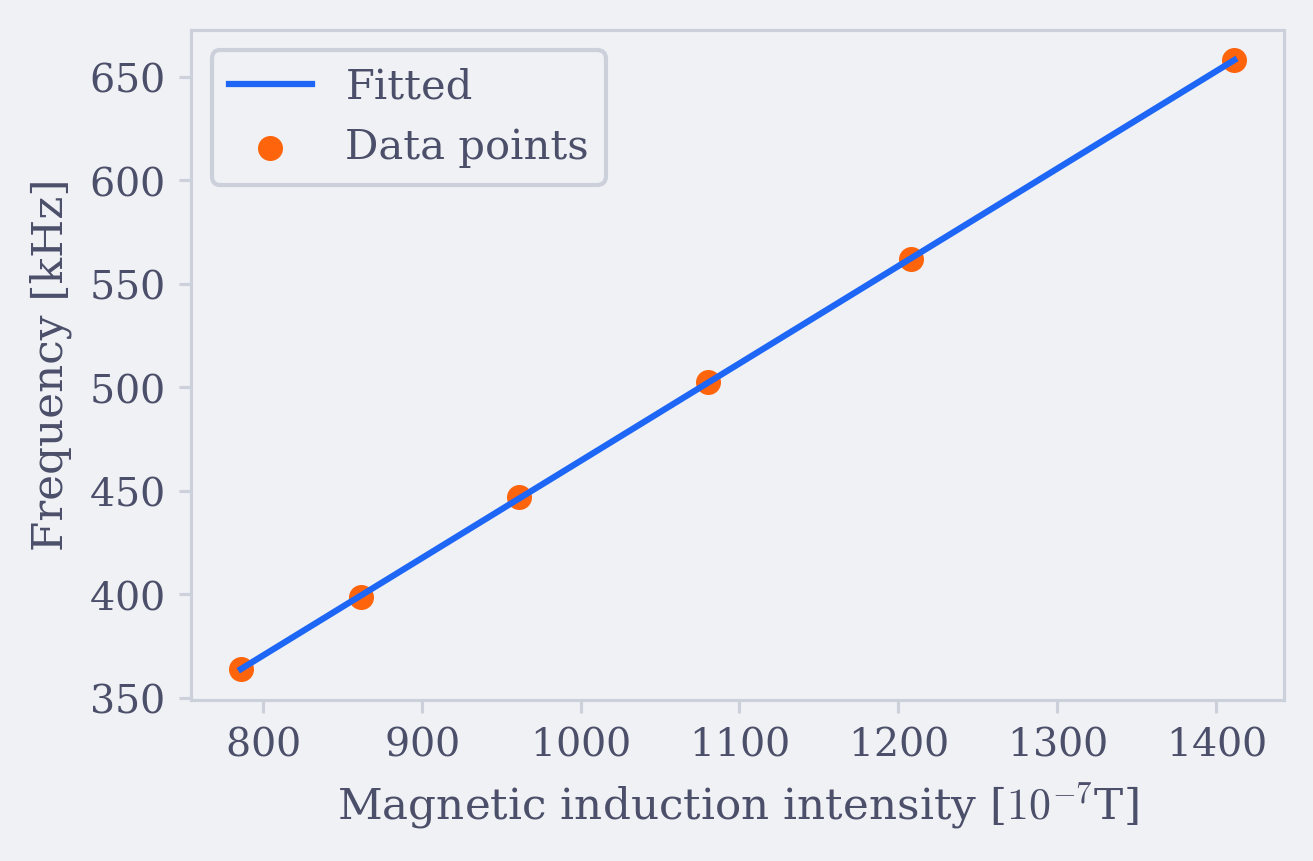
\includegraphics[width=0.9\linewidth]{ex4_1.png}
        \caption{$^{85}$Rb 拟合曲线}
        \label{fig:rb85}
    \end{minipage}
    \hfill
    \begin{minipage}{0.45\textwidth}
        \centering
        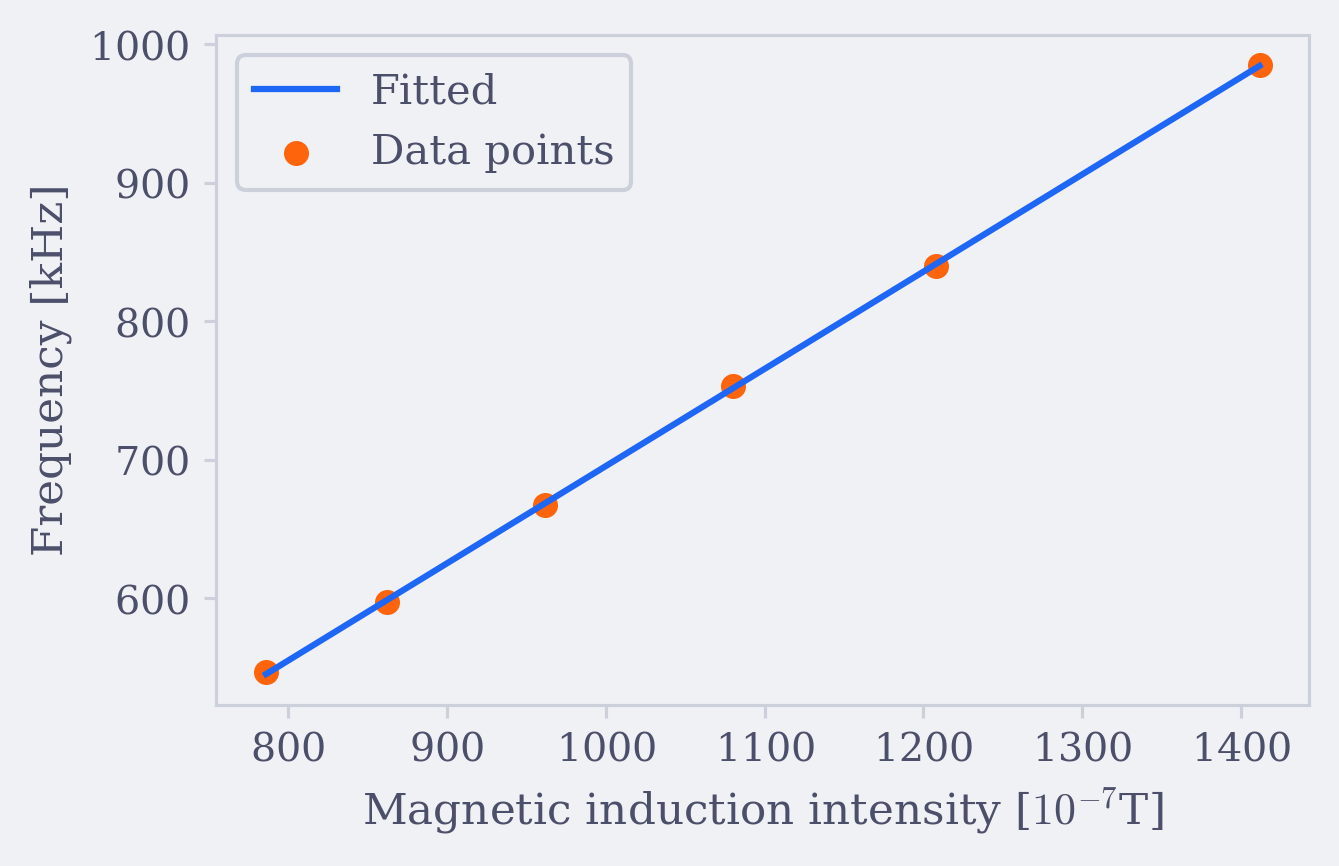
\includegraphics[width=0.9\linewidth]{ex4_2.png}
        \caption{$^{87}$Rb 拟合曲线}
        \label{fig:rb87}
    \end{minipage}
\end{figure}

\begin{table}[htbp]
    \centering
    \caption{水平磁场线圈电流与共振频率}
    \label{tab:data}
    \begin{tabular}{
        S[table-format=1.3] % 电流I列(3位小数)
        S[table-format=1.4] % B0列(4位小数)
        S[table-format=3.0] % v_1_87列(整数)
        S[table-format=3.0] % v_1_85列(整数)
        S[table-format=4.0] % v_2_87列(整数)
        S[table-format=3.0] % v_2_85列(整数)
        S[table-format=4.1] % 平均值列(1位小数)
        S[table-format=3.1] % 平均值列(1位小数)
    }
    \toprule
    {电流I/A} & {$B_0$/GS ($\times 10^{-4}$)} & {$v_{1}^{87}$(\si{\kilo\hertz})} & {$v_{1}^{85}$(\si{\kilo\hertz})} & {$v_{2}^{87}$(\si{\kilo\hertz})} & {$v_{2}^{85}$(\si{\kilo\hertz})} & {$\frac{v_{1}^{87}+v_{2}^{87}}{2}$(\si{\kilo\hertz})} & {$\frac{v_{1}^{85}+v_{2}^{85}}{2}$(\si{\kilo\hertz})} \\
    \midrule
    0.298 & 1.3829 & 782 & 523 & 1188 & 793 & 985.0 & 658.0 \\
    0.255 & 1.1834 & 634 & 423 & 1046 & 701 & 840.0 & 562.0 \\
    0.228 & 1.0581 & 550 & 367 & 956 & 638 & 753.0 & 502.5 \\
    0.203 & 0.9421 & 461 & 309 & 874 & 585 & 667.5 & 447.0 \\
    0.182 & 0.8446 & 393 & 261 & 802 & 536 & 597.5 & 398.5 \\
    0.166 & 0.7704 & 340 & 227 & 753 & 501 & 546.5 & 364.0 \\
    \bottomrule
    \end{tabular}
\end{table}

最终根据拟合结果给出,实验测得铷原子朗德$g$因子数据如下:

\begin{itemize}
    \item ${}^{85}\text{Rb}$测量值:$g_F = 0.3433 \pm 0.0009$
    \item ${}^{87}\text{Rb}$测量值:$g_F = 0.5121 \pm 0.0019$
\end{itemize}


\begin{ubox}
{如何区分$\nu^{85}$ 和 $\nu^{87}$}
    通过朗德$g$因子公式:

$$ 
g_{F} = g_{J} \cdot \frac{F(F+1) + J(J+1) - I(I+1)}{2F(F+1)} 
$$

由于${}^{87}\mathrm{Rb}$的核自旋$I=3/2$而${}^{85}\mathrm{Rb}$的$I=5/2$,计算可得:

$$ 
g_{F}^{87} > g_{F}^{85}
$$

根据共振频率公式:

$$ 
\nu = \frac{g_{F} \mu_{B} B_{0}}{h} 
$$

显然有:

$$ 
\nu^{87} > \nu^{85}
$$
\end{ubox}
\begin{ubox}
    {磁共振信号与光抽运信号的区别?}
    
\begin{enumerate}[label=(\arabic*), leftmargin=2em]
    \item \textbf{能量来源不同}
    \begin{itemize}[leftmargin=3em]
        \item 光抽运信号:能量来源于光能(如圆偏振光)
        \item 磁共振信号:能量来源于射频场电磁能 $E_{\text{rf}} = h\nu$ 和磁场能 $E_B = \mu_B B_0$
    \end{itemize}

    \item \textbf{实验条件不同}
    \begin{itemize}[leftmargin=3em]
        \item 光抽运信号:扫场速度需匹配原子弛豫时间 $\tau$($\Delta t \sim \tau$)
        \item 磁共振信号:射频频率需满足共振条件 $\nu = \dfrac{g_F \mu_B B_0}{h}$
    \end{itemize}

    \item \textbf{信号特征不同}
    \begin{itemize}[leftmargin=3em]
        \item 光抽运信号:
        \begin{itemize}
            \item 呈现指数型曲线 $I(t) = I_0(1-e^{-t/\tau})$
            \item 时间响应:慢变过程($\tau \sim \SI{1}{ms}$量级)
        \end{itemize}
        \item 磁共振信号:
        \begin{itemize}
            \item 呈现洛伦兹型共振峰 $\Delta I \propto \dfrac{1}{1+(\nu-\nu_0)^2 T_2^2}$
            \item 时间响应:瞬时响应($\Delta t \sim \SI{1}{\micro s}$量级)
        \end{itemize}
    \end{itemize}
\end{enumerate}

\end{ubox}
\subsubsection{误差分析}

\begin{itemize}[leftmargin=2em]
    \item ${}^{85}\text{Rb}$测量结果:$g_F = 0.3433 \pm 0.0009$(理论值$0.3334$)
    \item ${}^{87}\text{Rb}$测量结果:$g_F = 0.5121 \pm 0.0019$(理论值$0.4998$)
\end{itemize}
\begin{align*}
    \text{${}^{85}\text{Rb}$相对误差} &= \left|\frac{0.3433 - 0.3334}{0.3334}\right| \times 100\% \approx \SI{2.97}{\percent} \\
    \text{${}^{87}\text{Rb}$相对误差} &= \left|\frac{0.5121 - 0.4998}{0.4998}\right| \times 100\% \approx \SI{2.46}{\percent}
\end{align*}
误差来源分析:
\begin{enumerate}
    \item \textbf{磁场相关误差}:线圈几何参数的制造公差,电流测量设备的系统偏差’磁场空间分布的不均匀效应。
  
    
    \item \textbf{频率控制误差}:射频信号源的频率调节精度限制,参考时钟的长期稳定性问题。
    
    
    \item \textbf{电磁环境干扰}:实验室背景电磁噪声污染,仪器间电磁耦合导致的信号失真。
   
    \item \textbf{光学系统误差}:偏振光学元件的安装对准偏差,环境磁场补偿的残余分量。
   
    
    \item \textbf{温度效应误差}: 吸收池温度波动引起的信号漂移,温度敏感的系统响应特性变化
\end{enumerate}


\subsection{利用光泵磁共振方法测量地磁场}


\subsubsection{地磁场垂直分量$B_{E\perp}$的测量}

扫场信号使用方波信号,让垂直磁场与地磁场垂直分量方向相反,调节垂直线圈直流电流,改变垂直磁场大小,使得抽运信号幅度最大,此时的垂直磁场大小即为$B_{E\perp}$。

调节过程中,记录下不同垂直线圈电流$I_{\perp}$及对应的抽运信号幅度$V_{pp}$如下表:

\begin{table}[h]
\centering
\caption{垂直线圈电流与抽运信号幅度关系}
\label{tab:data_horizontal}
\begin{tabular}{*{13}{c}}
\toprule

$I_z$ (\si{\ampere})&0.013 & 0.020 & 0.025 & 0.030 & 0.035 & 0.040 & \textcolor{red}{0.041} & 0.045 & 0.050 & 0.055 & 0.060 & 0.065  \\
\midrule
$signal_z$ (V)&2.00 & 2.12 & 2.28 & 2.38 & 2.54 & 2.90 & \textcolor{red}{2.92} & 2.64 & 2.42 & 2.29 & 2.11 & 2.05  \\
\bottomrule
\end{tabular}
\end{table}



为获取信号最大时对应的电流值,对实验数据进行洛伦兹函数拟合,拟合函数形式为:
$$ \text{Lorentzian}(x; A, x_0, \gamma, B) = A \cdot \frac{\gamma^2}{(x - x_0)^2 + \gamma^2} + B $$

拟合结果参数如下:
\begin{itemize}
\item 振幅 $A = 0.9086$ V
\item 中心位置 $x_0 = 0.0406 \pm 0.0005$ \si{\ampere}
\item 半高宽 $\gamma = 0.0091$ \si{\ampere}
\item 基线偏移 $B = 1.9682$ V
\item 决定系数 $R^2 = 0.971469$
\end{itemize}
\begin{figure}[{H}]
    \centering
    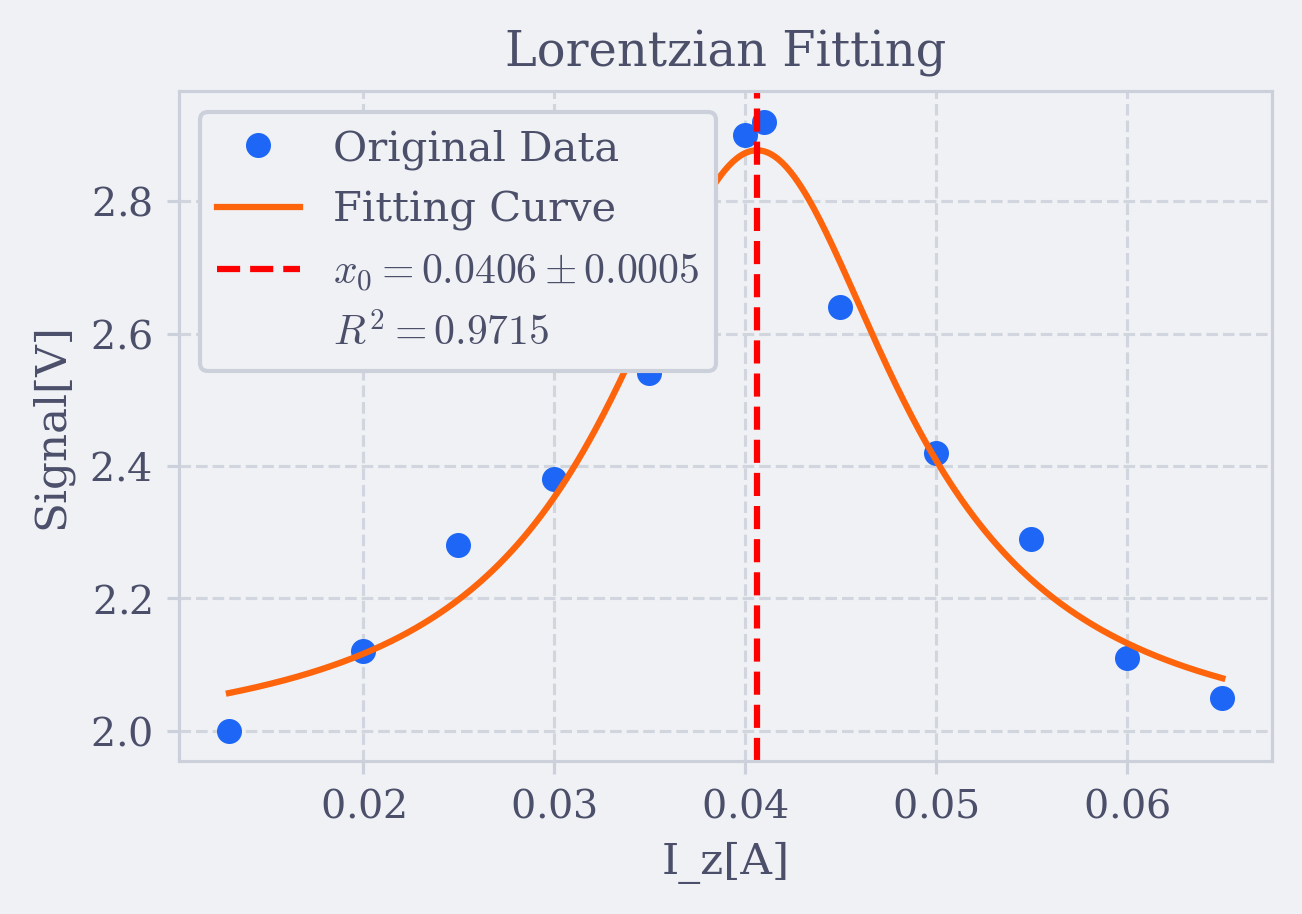
\includegraphics[width=0.7\linewidth]{ex5_2.png}
    \caption{拟合曲线}
    \label{}
\end{figure}

记录下光抽运信号最大时,垂直线圈的电流为\SI{0.0406}{\ampere},且两个垂直磁场线圈是串联的,数字表的电流是流过单个线圈的电流,电流需要乘2。根据公式:

$$ B = \frac{16\pi NI \times 10^{-7}}{5^{\frac{3}{2}} \cdot r} \, \text{(T)} $$

计算可得:
$$ B_{E\perp} = \SI{2.388567e-05}{\tesla} \pm \SI{3.054210e-07}{\tesla}$$

\subsubsection{地磁场水平分量$B_{E\parallel}$的测量}

    地磁场水平分量的测量方法:

    根据水平方向的总磁场:
    $$ B = B_{0} + B_{E_{\parallel}} + B_{S} $$

    调节扫场与其他两水平分量同向时:

    $$h \nu_{1} = g_{F} \mu_{B}(B_{0} + B_{E_{\parallel}} + B_{S}) $$

    调节扫场磁场与其他两水平分量反向时:

    $$h \nu_{2} = g_{F} \mu_{B}(B_{0} + B_{E_{\parallel}} - B_{S})$$


    最终得出如下关系:$$ B_{E_{\parallel}} = \frac{h}{g_F \mu_B} \cdot \frac{v_1 + v_2}{2}- B_{0}$$

    测量相关数据如表\ref{tab:current_freq}所示,根据数据进行拟合,得出如图\ref{fig:87fit}和图\ref{fig:85fit}的拟合结果。


\begin{table}[h]
\centering
\caption{地磁场水平分量测量,水平磁场线圈电流与共振频率数据}
\label{tab:current_freq}
\begin{tabular}{S[table-format=1.3] *{4}{S[table-format=3.0]}}
\toprule
{水平磁场电流 (\si{\ampere})} & {$\nu_1^{87}$ (\si{\kilo\hertz})} & {$\nu_1^{85}$ (\si{\kilo\hertz})} & {$\nu_2^{87}$ (\si{\kilo\hertz})} & {$\nu_2^{85}$ (\si{\kilo\hertz})} \\
\midrule
0.172 & 362 & 242 & 291 & 196 \\
0.193 & 358 & 239 & 430 & 288 \\
0.207 & 473 & 315 & 394 & 263 \\
0.214 & 421 & 282 & 498 & 333 \\
0.223 & 532 & 355 & 460 & 306 \\
0.236 & 498 & 333 & 573 & 382 \\
\bottomrule
\end{tabular}
\end{table}

对两组数据分别进行线性回归:

\begin{figure}[H]
\centering
\begin{minipage}{0.48\textwidth}
    \centering
    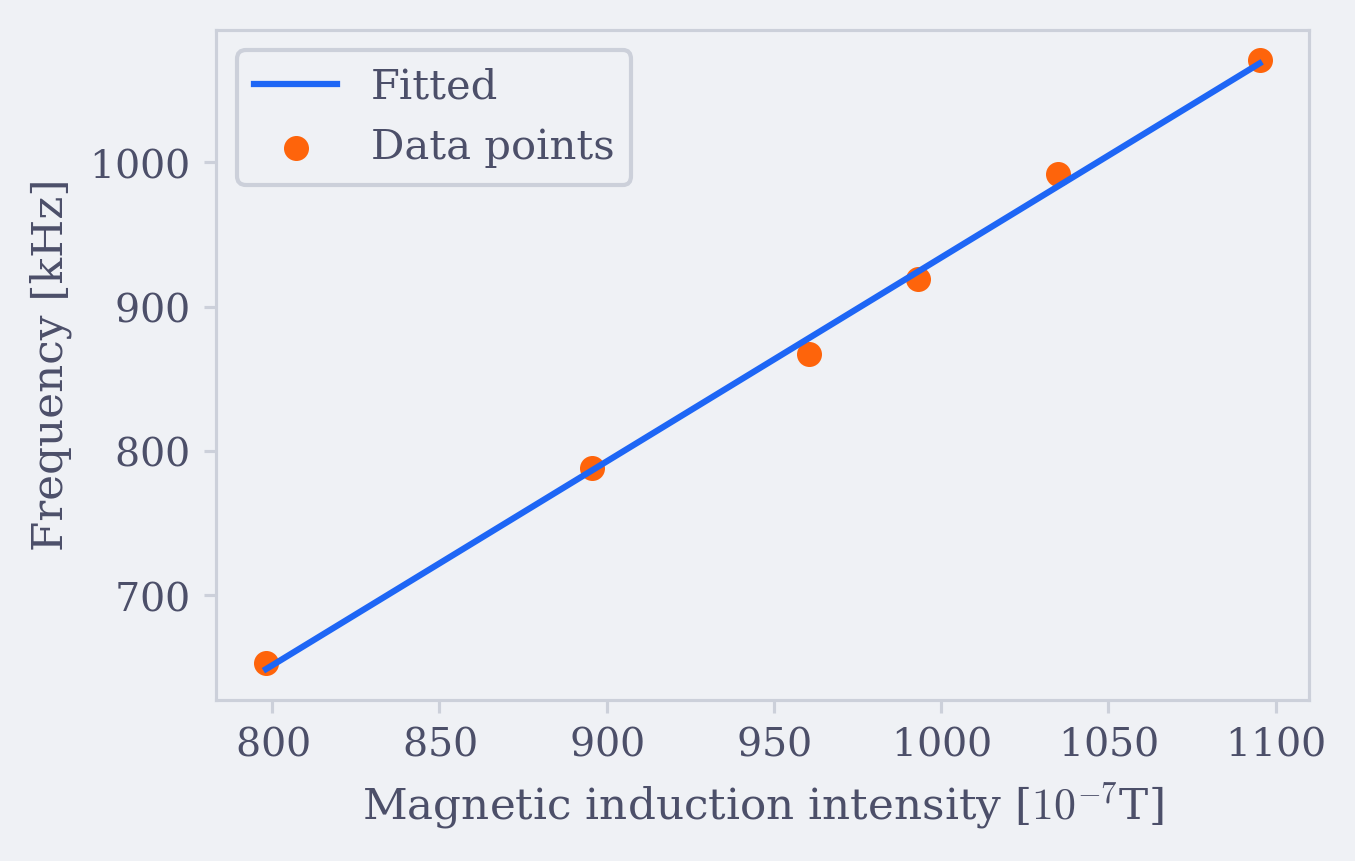
\includegraphics[width=\linewidth]{ex5_87.png}
    \caption{${}^{87}\text{Rb}$拟合曲线}
    \label{fig:87fit}
\end{minipage}
\hfill
\begin{minipage}{0.48\textwidth}
    \centering
    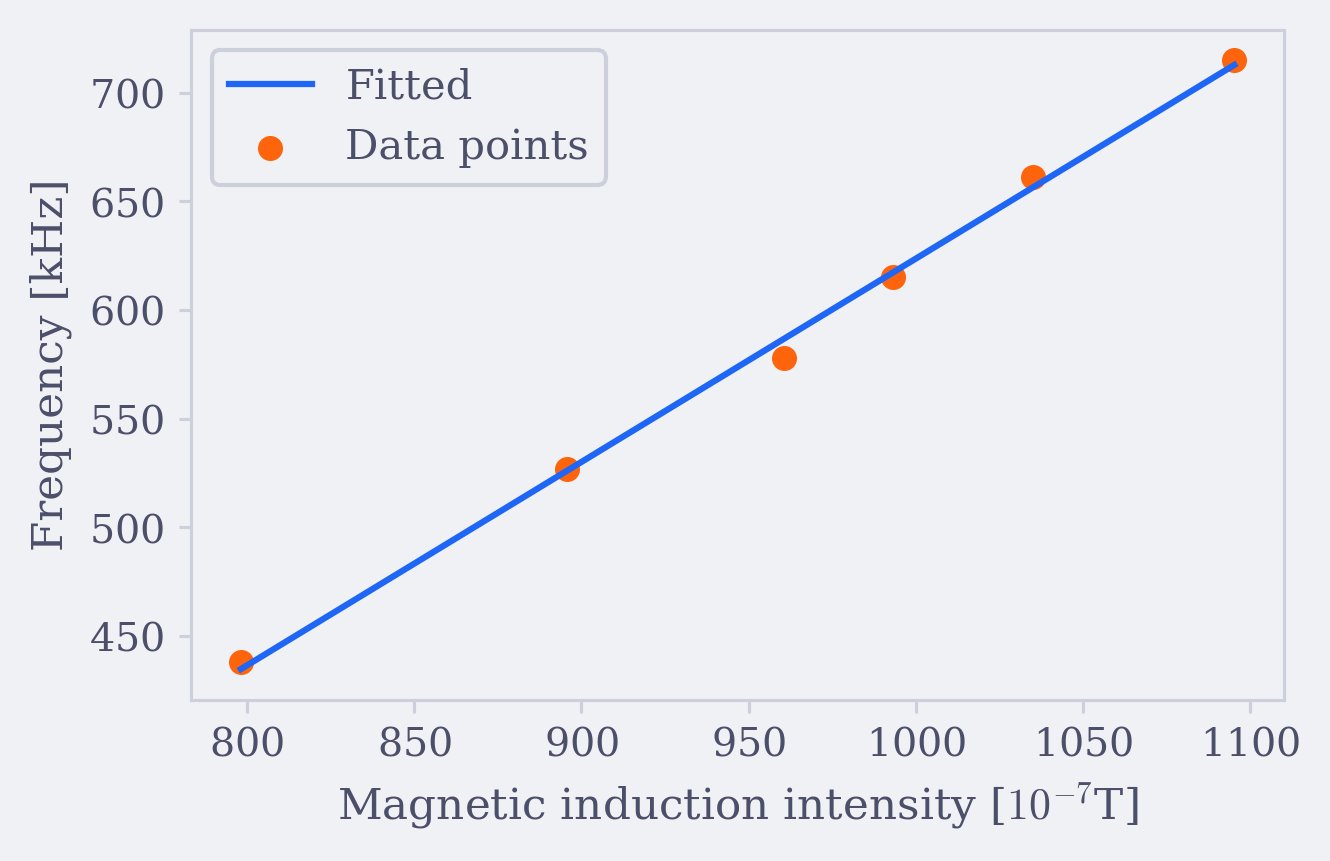
\includegraphics[width=\linewidth]{ex5_85.png}
    \caption{${}^{85}\text{Rb}$拟合曲线}
    \label{fig:85fit}
\end{minipage}
\end{figure}
\begin{itemize}
\item ${}^{87}\text{Rb}$拟合结果计算得出:$B_{87} = \SI{3.463236e-5}{\tesla} \pm \SI{2.530420e-6}{\tesla}$
\item ${}^{85}\text{Rb}$拟合结果计算得出:$B_{85} = \SI{3.404010e-5}{\tesla} \pm \SI{2.610477e-6}{\tesla}$
\end{itemize}

取两组测量结果的平均值:
$$
B_{xy} = \frac{B_{87} + B_{85}}{2} = \SI{3.433623e-05}{\tesla} \pm \SI{1.817802e-06}{\tesla}
$$

\subsubsection{地磁场测量结果}

\begin{itemize}
    \item 水平分量:$B_{xy} = \SI{3.433623e-05}{\tesla} \pm \SI{1.817802e-06}{\tesla}$(取${}^{87}\text{Rb}$和${}^{85}\text{Rb}$平均值)
    \item 垂直分量:$B_z = \SI{2.388567e-05}{\tesla} \pm \SI{3.054210e-07}{\tesla}$(由拟合结果电流\SI{0.0406}{\ampere}计算)
    \item 总磁场强度:$B_{\text{earth}} = \sqrt{B_{xy}^2 + B_z^2} = \SI{4.182705e-05}{\tesla} \pm \SI{1.502409e-06}{\tesla}$
    \item 地磁倾角:$\theta = \arctan\left(\frac{B_z}{B_{xy}}\right) = \SI{34.82}{\degree} \pm \SI{1.46}{\degree}$
\end{itemize}

标准参考值为:
\begin{itemize}
    \item 总磁场强度:$B_{\text{ref}} = \SI{45595.2}{\nano\tesla} = \SI{45.5952}{\milli\tesla}$
    \item 地磁倾角:$\theta_{\text{ref}} = \ang{33;58} \approx \SI{33.9667}{\degree}$
\end{itemize}

误差分析:
\begin{align*}
    \text{磁感应强度相对误差} &= \left|\frac{41.8127 - 45.5952}{45.5952}\right| \times 100\% \approx \SI{8.30}{\percent} \\
    % \text{地磁倾角绝对误差} &= \SI{35.3464}{\degree} - \SI{33.9667}{\degree} = \SI{1.3797}{\degree} \\
    \text{倾角相对误差} &= \left|\frac{34.82 - 33.9667}{33.9667}\right| \times 100\% \approx \SI{2.51}{\percent}
\end{align*}

误差来源分析:
\begin{enumerate}
    \item 水平分量测量中${}^{87}\text{Rb}$与${}^{85}\text{Rb}$的\SI{1.7}{\percent}差异
    \item 垂直方向电流\SI{0.0406}{\ampere}的标定误差
    \item 线圈半径$r=\SI{0.1530}{\meter}$的制造公差
\end{enumerate}



\subsection{研究不同偏振态的光对光抽运信号强度的影响}


\subsubsection{1/4 玻片对光束偏振态的调制机理}
实验中采用D1$\sigma^+$偏振光作为入射光,其作用是将铷原子抽运到基态$5^2S_{1/2}$超精细结构的$F=2,m_F=+2$塞曼子能级上。1/4波片在快慢轴间引入$\pi/2$相位延迟,其琼斯矩阵表示为:

$$ \mathbf{J}_{\lambda/4}(\theta) = R^{T}(\theta)\cdot
\begin{pmatrix}
1 & 0 \\
0 & i 
\end{pmatrix}
\cdot R(\theta) = 
\begin{pmatrix}
\cos^2\theta + i\sin^2\theta & (1-i)\sin\theta\cos\theta \\
(1-i)\sin\theta\cos\theta & \sin^2\theta + i\cos^2\theta
\end{pmatrix} $$

对于初始线偏振光$\mathbf{E}_i = E_0\begin{pmatrix} \cos\alpha \\ \sin\alpha \end{pmatrix}$,出射光场为:

$$ \mathbf{E}_o = \mathbf{J}_{\lambda/4}(\theta)\mathbf{E}_i = E_0
\begin{pmatrix}
\cos(\theta-\alpha)\cos\theta + i\sin(\theta-\alpha)\sin\theta \\
\cos(\theta-\alpha)\sin\theta - i\sin(\theta-\alpha)\cos\theta
\end{pmatrix} $$

当$\theta-\alpha=45^\circ$时,出射光满足$|E_{ox}|=|E_{oy}|$且相位差$\Delta\phi=\pi/2$,形成完美圆偏振光:

$$ \mathbf{E}_o\big|_{\theta=45^\circ} = \frac{E_0}{\sqrt{2}}
\begin{pmatrix}
1 \\
i 
\end{pmatrix} \quad \text{(右旋圆偏振)} $$

信号强度与角度的关系为:

$$ S(\theta) = S_{\text{max}}\left|\frac{E_{ox}-iE_{oy}}{\sqrt{2}}\right|^2 = \frac{S_{\text{max}}}{2}[1+\sin(4\theta)] $$

\begin{itemize}

\item 典型角度下的偏振态:
\begin{align*}
&\theta=0^\circ: \quad \mathbf{E}_o = E_0\begin{pmatrix} 1 \\ 0 \end{pmatrix} \quad \text{(x方向线偏振)} \\
&\theta=45^\circ: \quad \mathbf{E}_o = \frac{E_0}{\sqrt{2}}\begin{pmatrix} 1 \\ i \end{pmatrix} \quad \text{(右旋圆偏振)} \\
&\theta=22.5^\circ: \quad \mathbf{E}_o = E_0\begin{pmatrix} \cos\frac{\pi}{8} \\ i\sin\frac{\pi}{8} \end{pmatrix} \quad \text{(椭圆偏振)}
\end{align*}
\end{itemize}
\subsubsection{测量结果与拟合分析}
测量得出如下数据:

\begin{table}[htbp]
\centering
\caption{角度-信号强度对应关系测量数据(双周期对比)}
\label{tab:angle-voltage-8col}
\footnotesize
\begin{tabular}{
    S[table-format=3.0]  % 周期1角度
    S[table-format=1.2]   % 周期1信号强度
    @{\hspace{1em}}      % 列间距
    S[table-format=3.0]  % 周期2角度
    S[table-format=1.2]   % 周期2信号强度
    S[table-format=3.0]  % 周期1角度
    S[table-format=1.2]   % 周期1信号强度
    @{\hspace{1em}}      % 列间距
    S[table-format=3.0]  % 周期2角度
    S[table-format=1.2]   % 周期2信号强度
}
\toprule
\multicolumn{2}{c}{\textbf{周期1}} & \multicolumn{2}{c}{\textbf{周期1}} & 
\multicolumn{2}{c}{\textbf{周期2}} & \multicolumn{2}{c}{\textbf{周期2}} \\
\cmidrule(r){1-2} \cmidrule(lr){3-4} \cmidrule(lr){5-6} \cmidrule(l){7-8}
{角度/\si{\degree}} & {信号强度/\si{V}} & {角度/\si{\degree}} & {信号强度/\si{V}} & 
{角度/\si{\degree}} & {信号强度/\si{V}} & {角度/\si{\degree}} & {信号强度/\si{V}} \\
\midrule
0    & 1.26 & 180  & 0.90 & 345  & 2.90 & 165  & 2.58 \\
15   & 2.10 & 195  & 1.98 & 330  & 2.58 & 150  & 3.12 \\
30   & 2.26 & 210  & 2.58 & 315  & 1.50 & 135  & 2.52 \\
45   & 1.58 & 225  & 1.94 & 300  & 0.30 & 120  & 1.14 \\
60   & 0.32 & 240  & 0.58 & 285  & 0.32 & 105  & 0.18 \\
75   & 0.14 & 255  & 0.10 & 270  & 1.82 & 90   & 0.60 \\
90   & 1.20 & 270  & 0.82 & 255  & 2.90 & 75   & 2.42 \\
105  & 2.50 & 285  & 2.10 & 240  & 2.82 & 60   & 3.28 \\
120  & 2.56 & 300  & 2.58 & 225  & 1.74 & 45   & 2.70 \\
135  & 1.84 & 315  & 2.18 & 210  & 0.94 & 30   & 1.52 \\
150  & 0.46 & 330  & 0.74 & 195  & 0.26 & 15   & 0.20 \\
165  & 0.10 & 345  & 0.20 & 180  & 0.70 & 0    & 0.42 \\
     &      & 360  & 1.28 &      &      &      &      \\
\bottomrule
\end{tabular}
\end{table}

\begin{figure}[{H}]
    \centering
    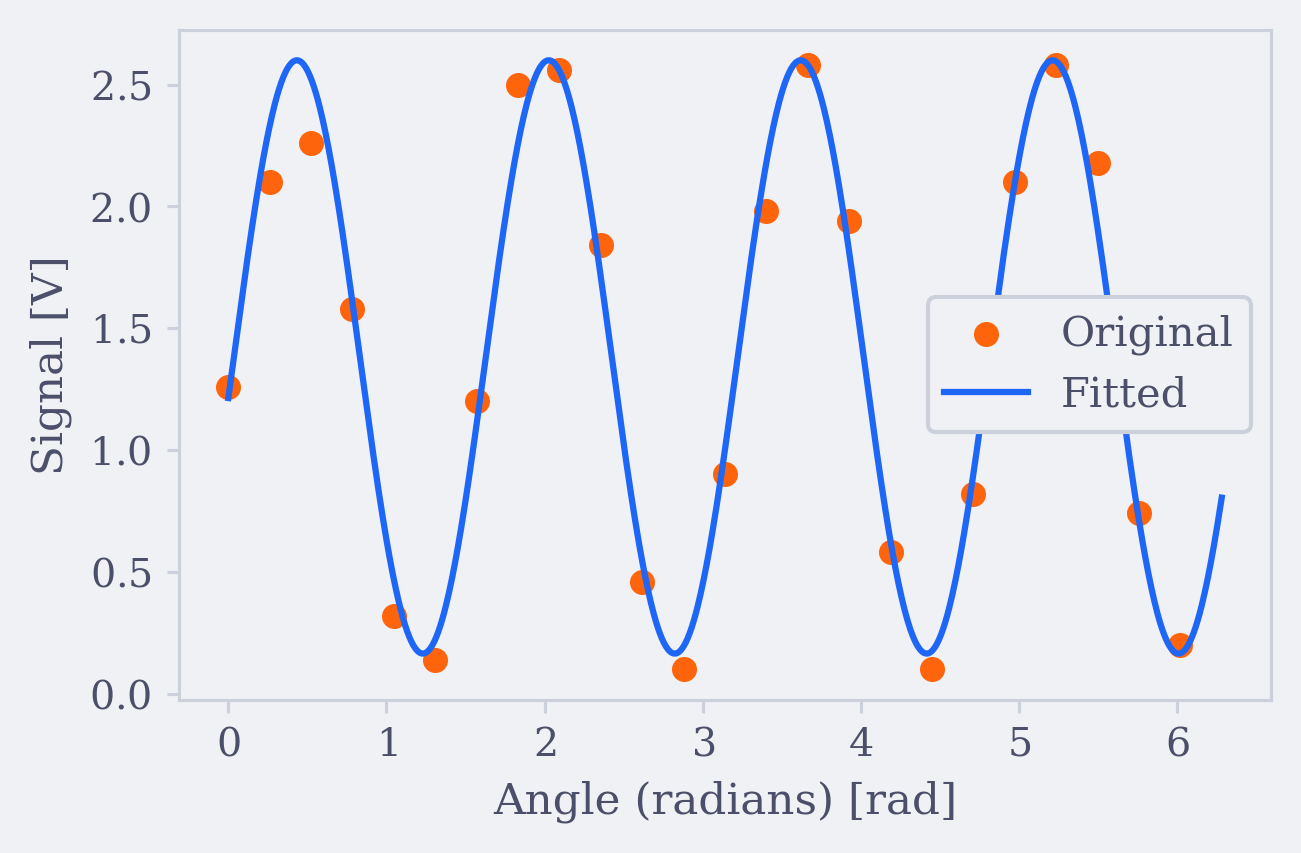
\includegraphics[width=0.5\linewidth]{ex6.png}
    \caption{拟合曲线}
    \label{}
\end{figure}

拟合参数
\begin{align*}
    A &= 1.217590 \pm 0.049880 \\
    \omega &= 3.943445 \pm 0.020722 \\
    \phi &= -0.138968 \pm 0.075250 \\
    C &= 1.382204 \pm 0.034878
\end{align*}

% 误差分析

% \begin{itemize}
%     \item 平均残差: \(-1.132894 \times 10^{-13}\)
%     \item 残差标准差: \(1.594824 \times 10^{-1}\)
%     \item 均方根误差 (RMSE): \(1.594824 \times 10^{-1}\)
% \end{itemize}


相关系数为$R^2 = 0.966049$,拟合效果很好,结合图像来看,振幅随角度的变化整体上符合理论预期。误差来源主要为光学器件转动角度的读取精度不高,读数不够精确,此外信号噪声同样会对读数结果产生影响。



\subsubsection{分析讨论}

    在本实验中,我们测量了不同角度下1/4波片调制出的偏振光对铷原子光抽运信号的影响。通过对比两周期内的信号强度变化,可以明显观察到随波片角度变化,抽运信号呈现明显的周期性波动,这与偏振态的变化规律密切相关。

    \begin{enumerate}
        \item 由\cref{tab:angle-voltage-8col}可知,信号强度形成一个90°为周期的波动规律;而1/4波片对线偏振光的调制效果为:每旋转180°,输出偏振态经历一次完整变化( $\sigma^+$→ 线偏振 → $\sigma^-$ → 线偏振 → $\sigma^+$)。说明在光抽运信号强度上,$\sigma^+$与$\sigma^-$并无明显差异。
        
        \item 而每90°一个周期会出现一次信号强度最小值,与线偏振光出现的频率相符,说明线偏振光无法持续积累定向态,几乎无法形成抽运信号。
    \end{enumerate}


\clearpage


\JMSection{实验后思考题}
\begin{question}
1. 理论分析如何利用偏振片和1/4波片获得圆偏振光?在改变入射光偏振状态的过程中,如何判断入射光接近圆偏振光?
\end{question}


要产生圆偏振光,需要使线偏振光的偏振方向与1/4波片光轴成$45^\circ$角。此时o光和e光振幅相等且产生$\pi/2$相位差,合成后形成圆偏振光。当夹角为$0^\circ$或$90^\circ$时,出射光仍为线偏振光;其他角度则产生椭圆偏振光。

判断圆偏振光可通过光抽运效应实现。圆偏振光($\sigma^+$或$\sigma^-$)会将原子抽运到特定磁子能级(如$m_F=+2$),产生最强抽运信号。线偏振光因$\sigma^+$和$\sigma^-$成分抵消而信号最弱,椭圆偏振光信号强度介于两者之间。当检测到最大抽运信号时,即可确认入射光接近圆偏振态。

\begin{question}
2. 能否利用D2 $\sigma^+$光对铷进行光抽运?为什么?
\end{question}


D2线($5^2S_{1/2}\rightarrow5^2P_{3/2}$)不适合高效光抽运。这是因为$5^2P_{3/2}$激发态的$J=3/2$导致其有四个超精细能级,原子在自发辐射时会以非均匀分支比返回多个基态子能级,破坏偏极化效果。

相比之下,D1线($5^2S_{1/2}\rightarrow5^2P_{1/2}$)因其$J=1/2$特性,仅有两个超精细能级($F'=I\pm1/2$),使用$\sigma^+$光时原子可被有效抽运到$m_F=+2$能级。D2线的复杂跃迁路径会导致部分原子返回低$m_F$态,显著削弱光抽运效率。


\begin{question}
3. 当垂直磁场方向不为零且扫场不过零,能否观察到光抽运信号?在这种条件下,试分析示波器显示的光吸收信号形成原因。
\end{question}


即使存在非零垂直磁场且扫场不过零,仍可能观测到光抽运信号,但信号强度会减弱且形态异常。这是因为残余磁场分量会改变塞曼能级分裂方式,影响原子的抽运和弛豫过程。

示波器显示的光吸收信号主要来源于两个机制:一是静态塞曼分裂导致部分能级仍可发生选择定则允许的跃迁;二是扫场分量使系统产生非平衡态布居。当垂直磁场较小时,可能观察到畸变的光抽运曲线;若磁场过强,则可能仅检测到恒定吸收背景或杂乱波动。


\begin{question}
4. 实现塞曼能级间的磁共振条件是什么?如何区别磁共振信号与光抽运信号?
\end{question}


磁共振需要满足能量匹配条件$\Delta E = h\nu$,即射频光子能量等于塞曼能级间距。对于$^{87}$Rb原子,当外加磁场$B$使塞曼分裂$\Delta E=g_F\mu_B B$与射频频率$\nu$匹配时即发生共振。

区分两类信号:磁共振信号是射频诱导的能级跃迁,表现为尖锐的共振峰,与磁场过零点无关;而光抽运信号是磁场过零时原子布居数重新分布的结果,呈现先下降后恢复的缓变曲线。






